\documentclass[]{article}

\usepackage{tikz}
\usepackage{graphicx}
\frenchspacing

\begin{document}

\title{Verslag Meeting 1}
\author{Axel Faes \and Matthijs Kaminski}
\date{26 januari 2015}
\maketitle

\section{Aanwezigheden}
\begin{itemize}
\item Raf Van Ham
\item Jonny Daenen
\item Axel Faes
\item Matthijs Kaminski
\end{itemize}

\section{Voorbereiding van meeting}
Het idee dat gevormd werd na het ontvangen van de projectopgave was een IDE die sterk gebasseerd was op de programmeeromgeving van Scratch. Als persoonlijke touch hadden we het idee voor een flow-based omgeving te creeeren. Hierbij zouden verschillende events van een sprite kunnen worden gekoppeld aan een functie-blok. Het doel van deze aanpak is om de flow en opvolging van de uitvoering duidelijker te maken voor de gebruiker (zonder dat deze over enige technische ervaring beschikt). \\\\
Hieronder volgen enkele mockups:\\\\
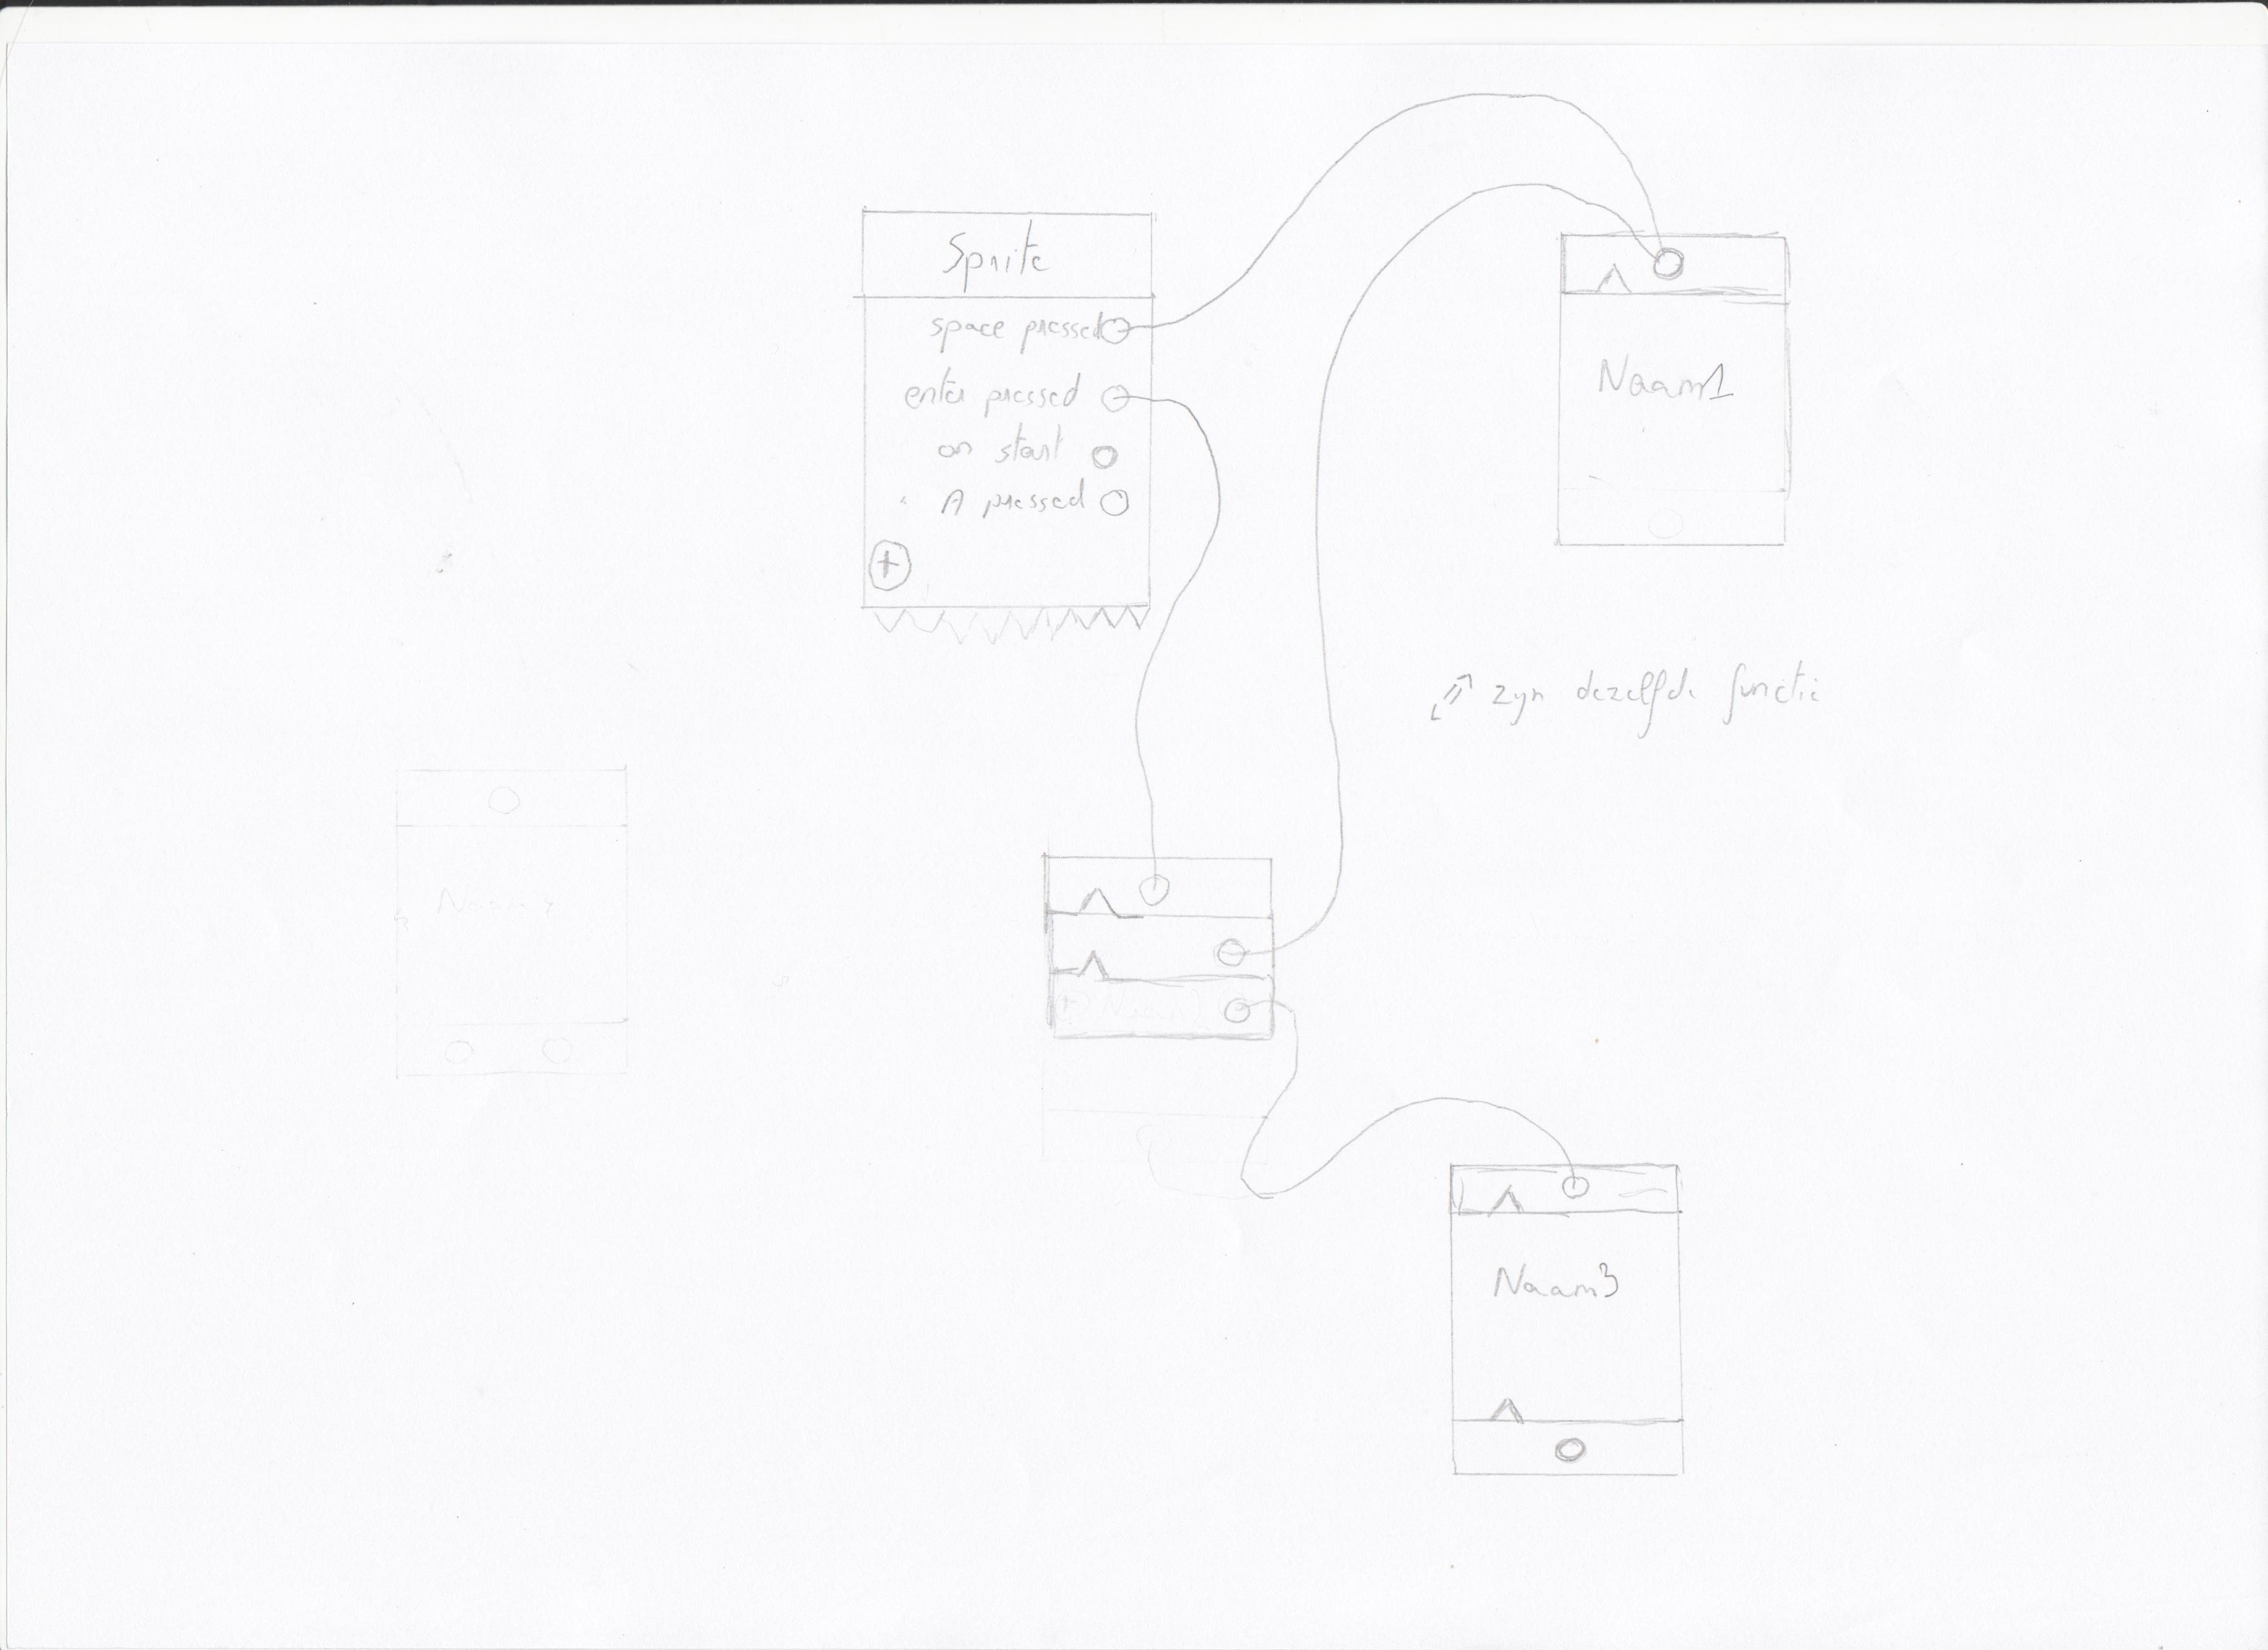
\includegraphics[scale=0.10]{mockup1-1.jpg}
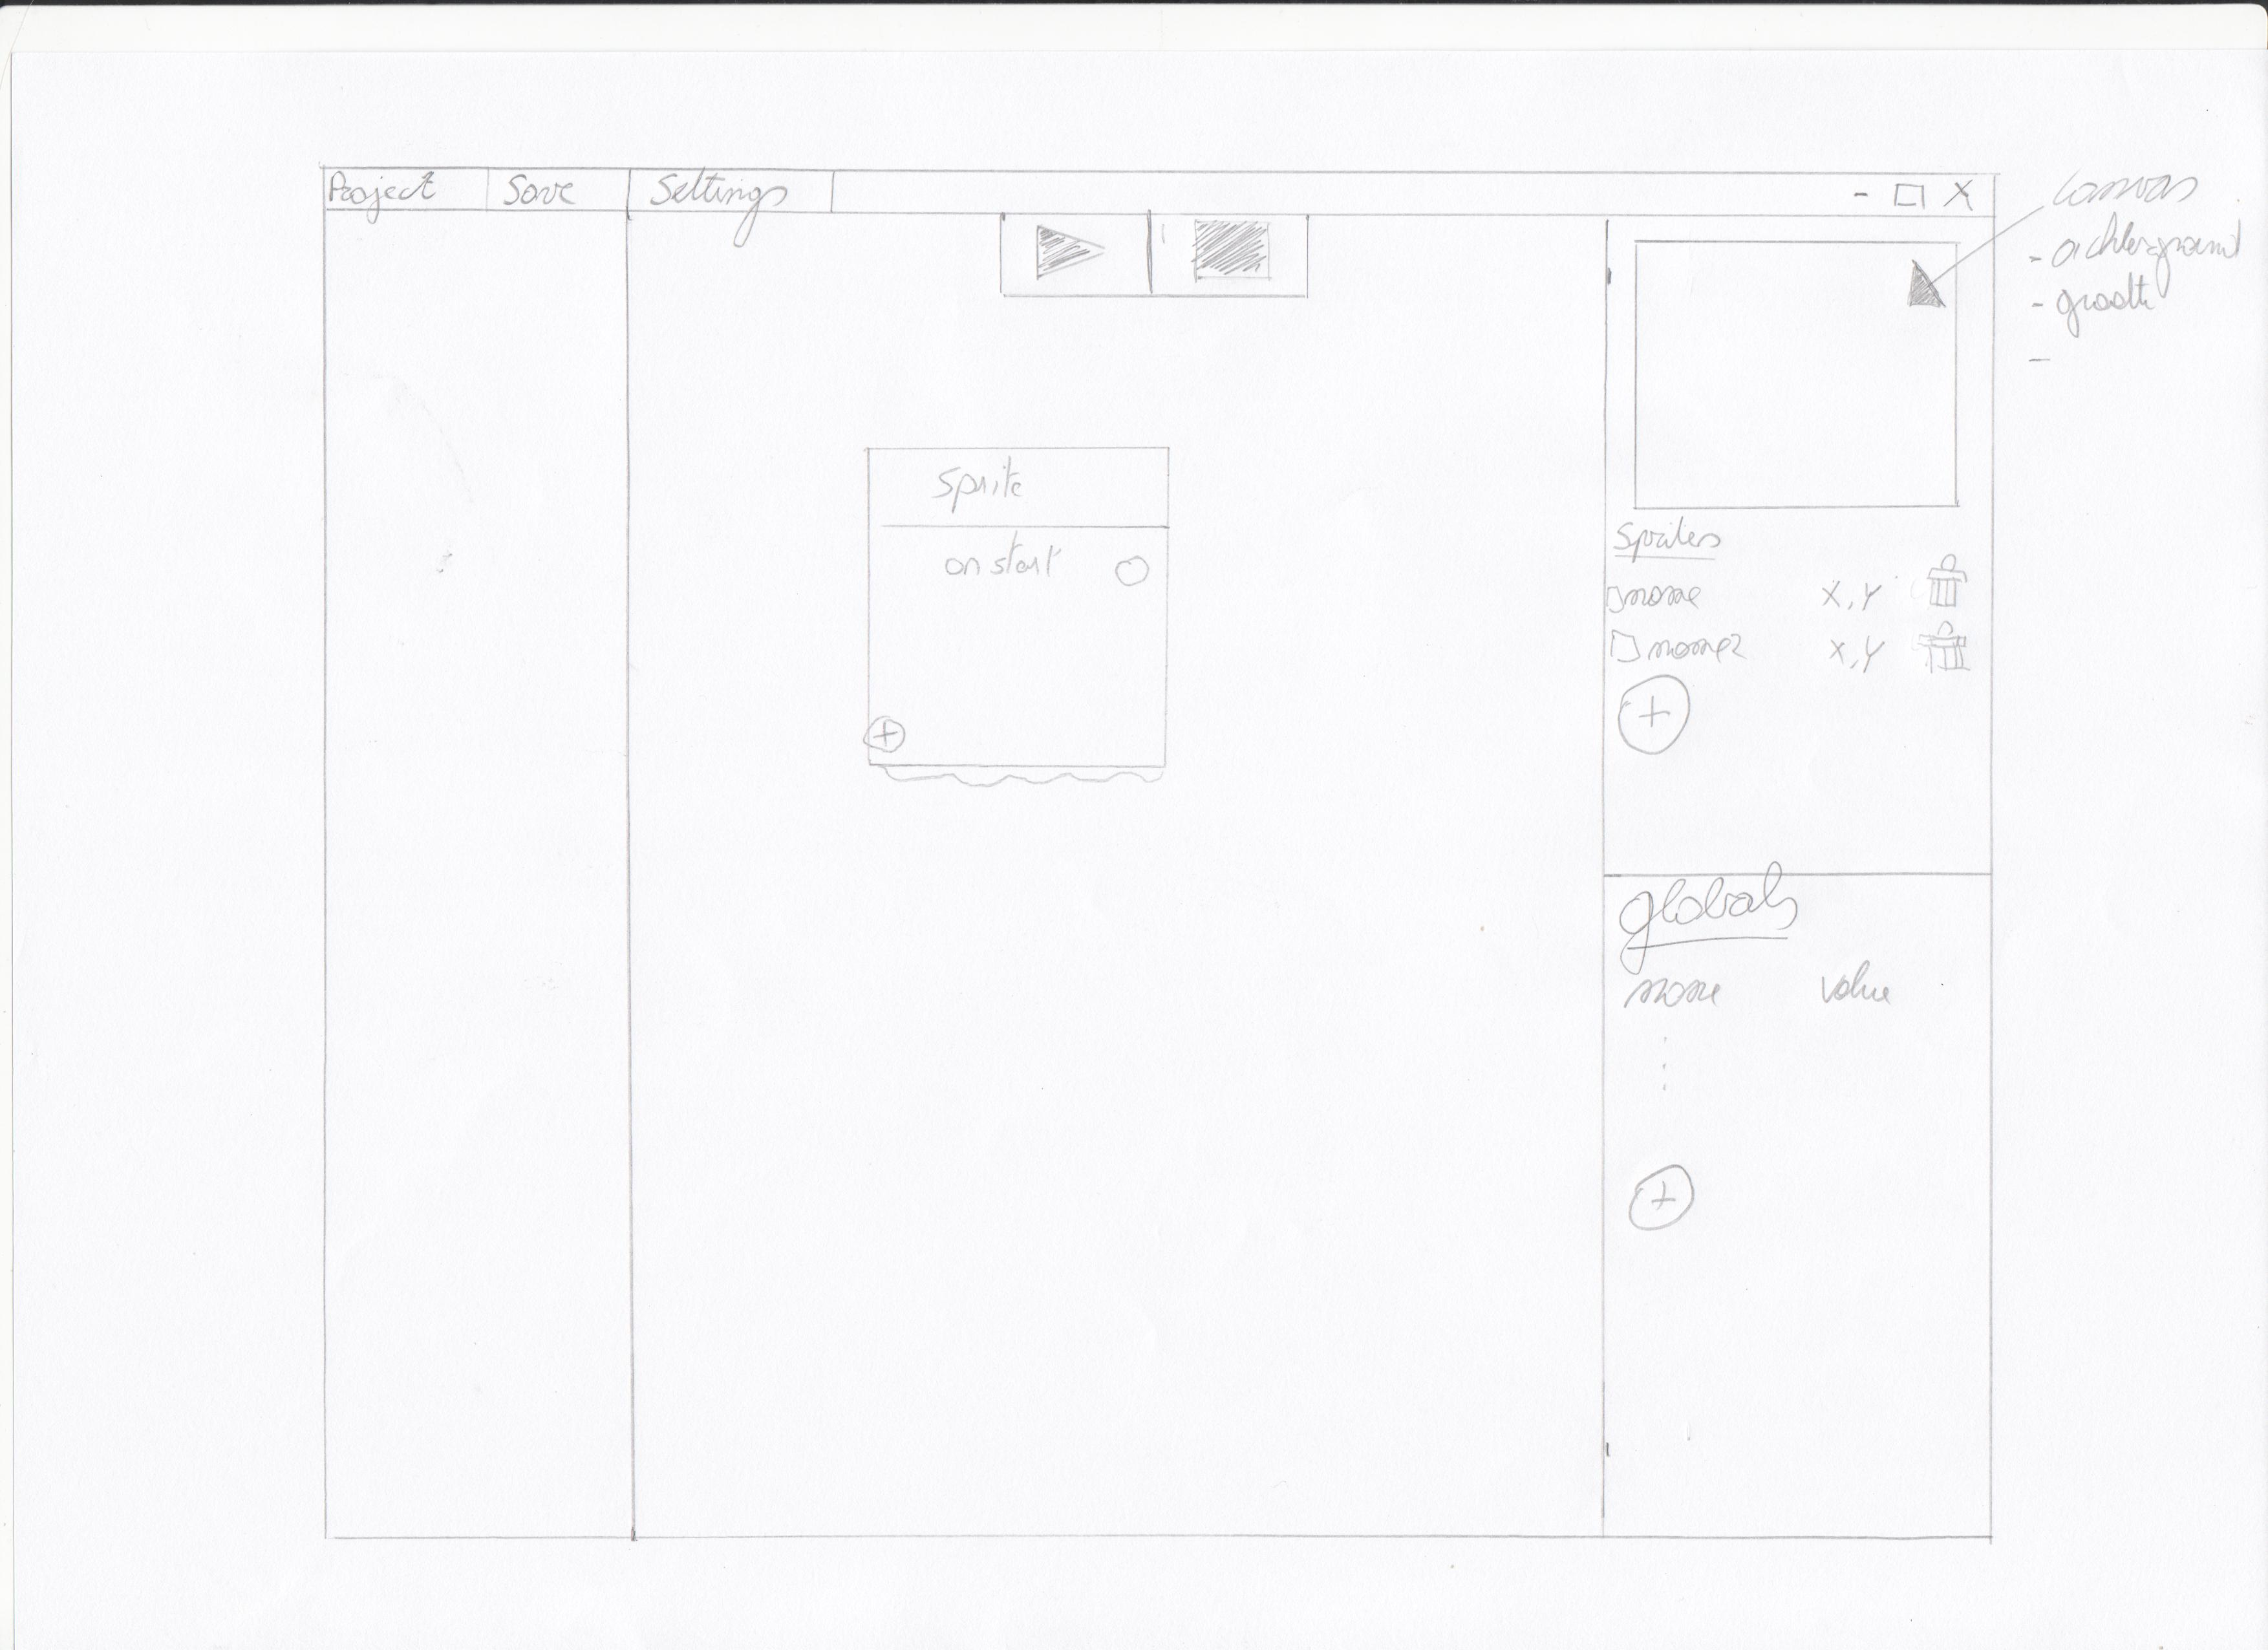
\includegraphics[scale=0.10]{mockup1-2.jpg}
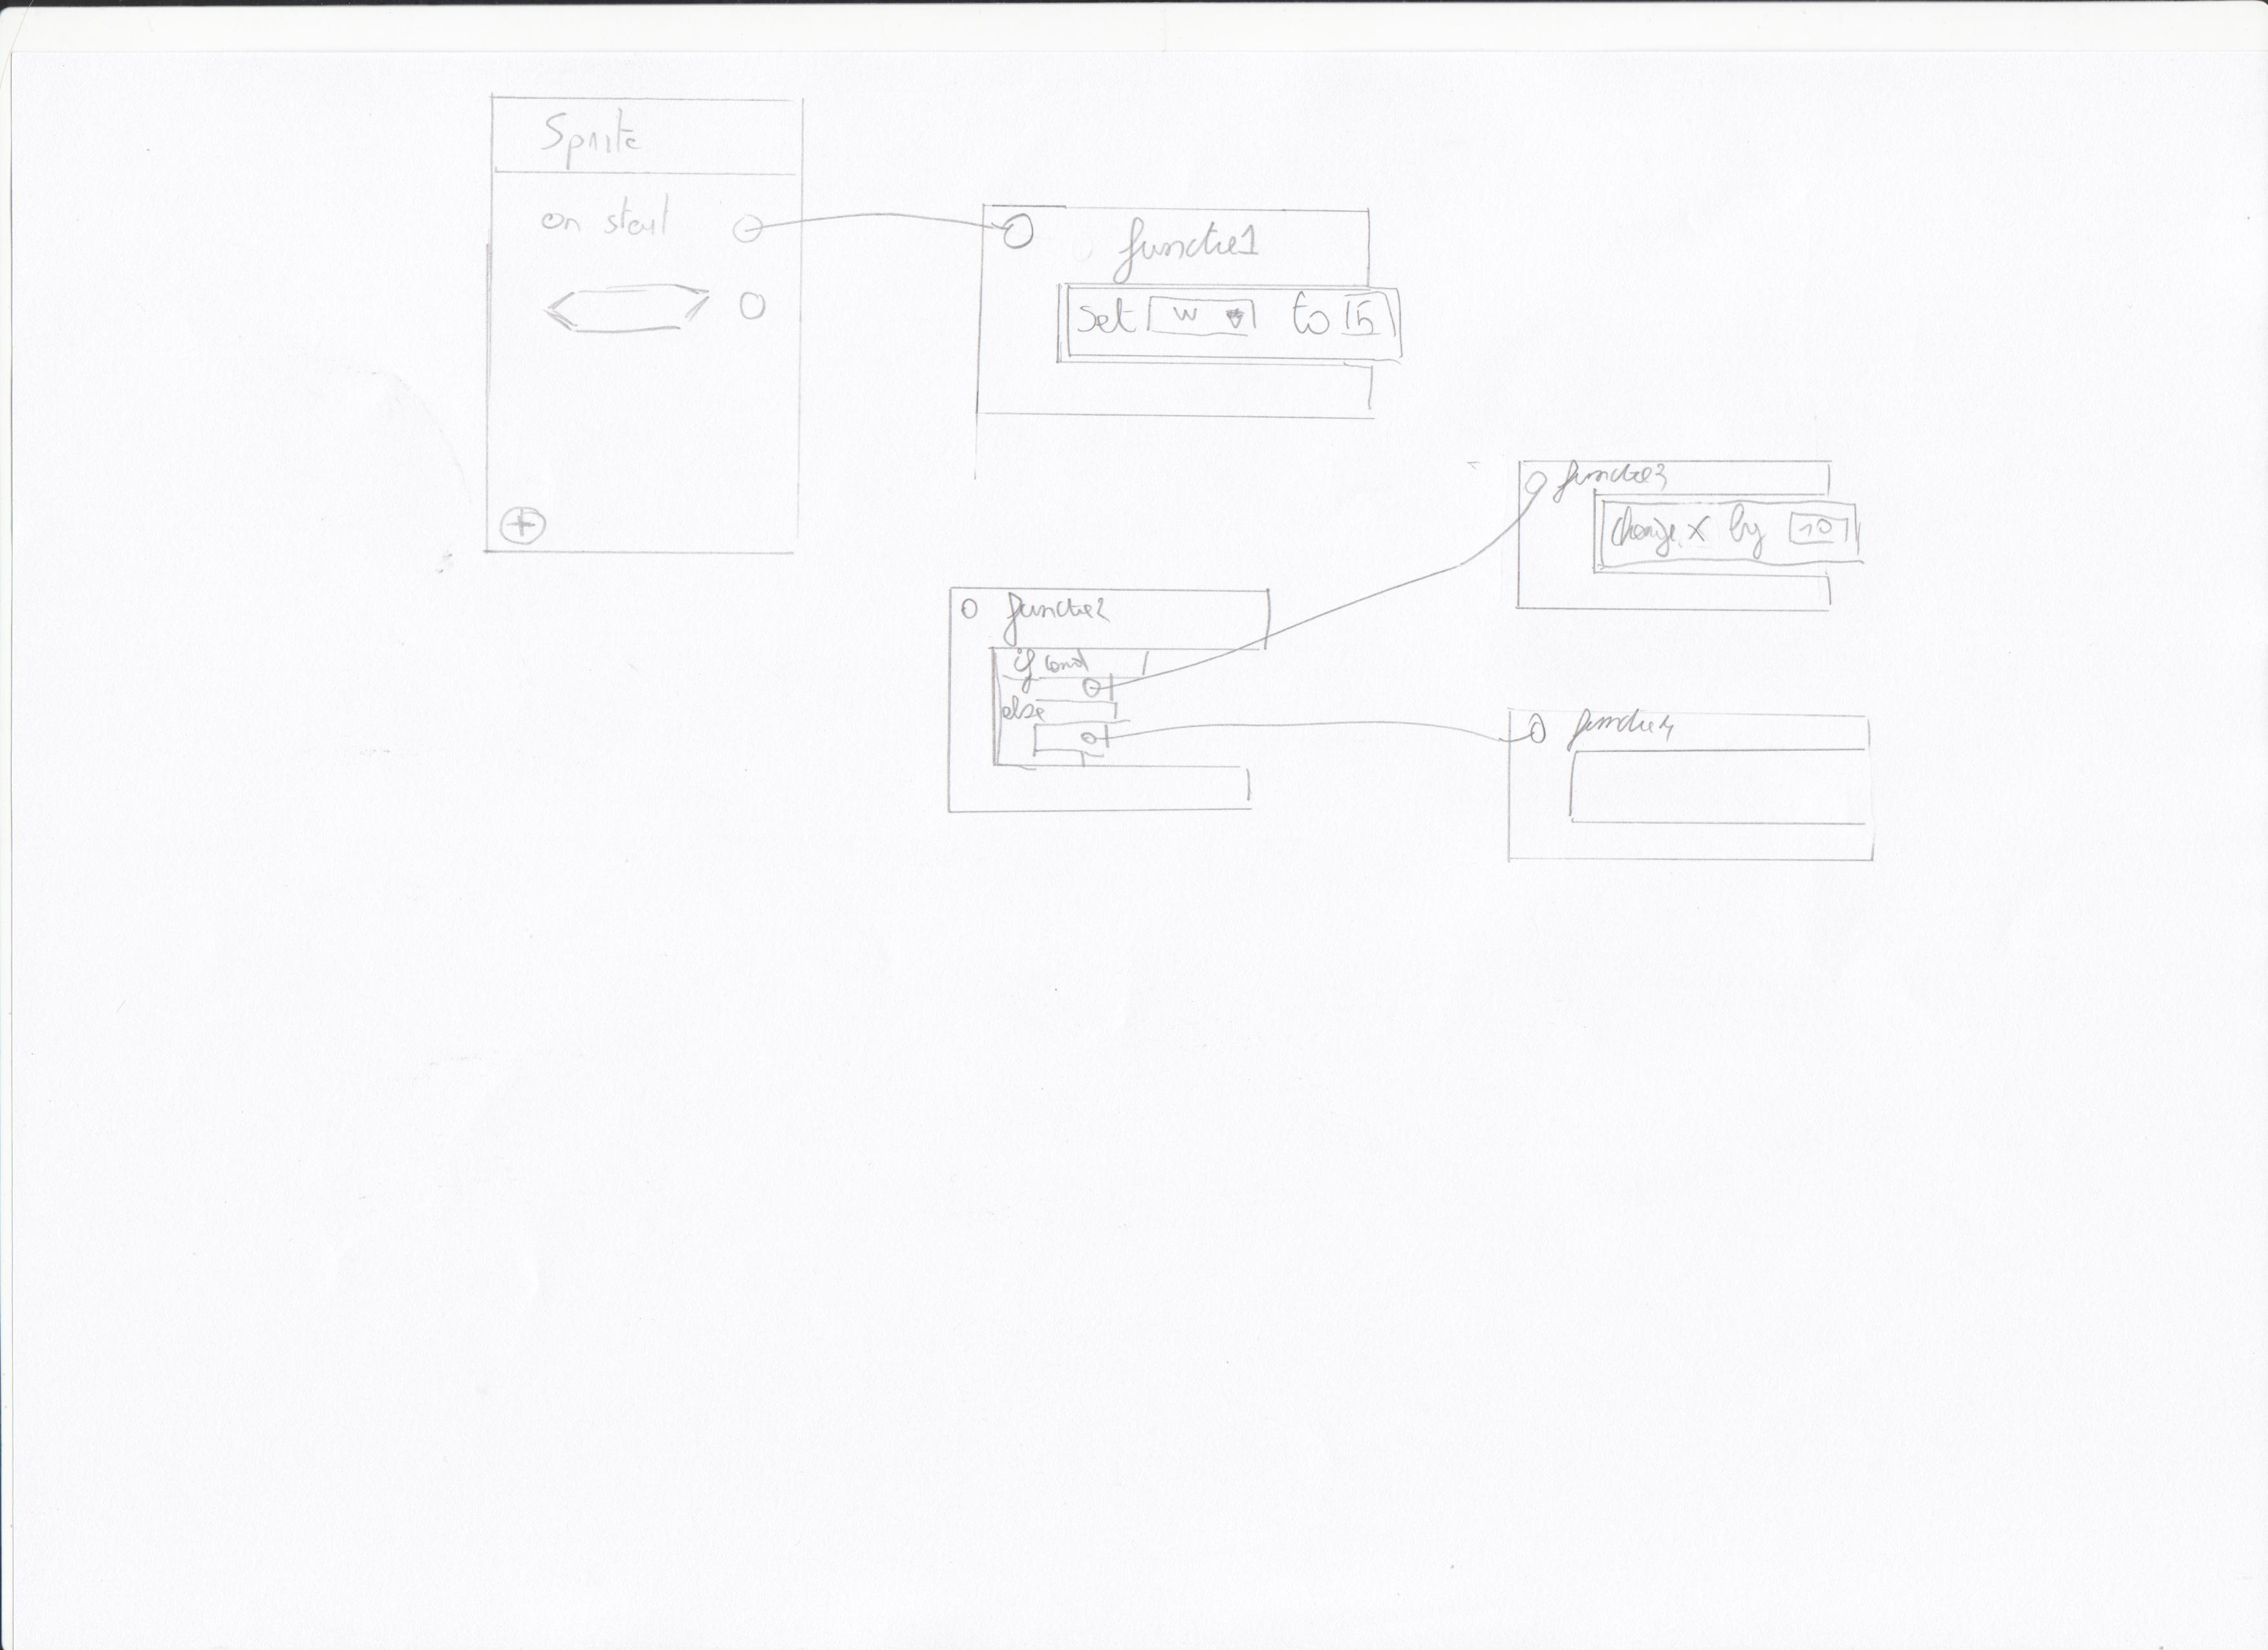
\includegraphics[scale=0.10]{mockup2-2.jpg}
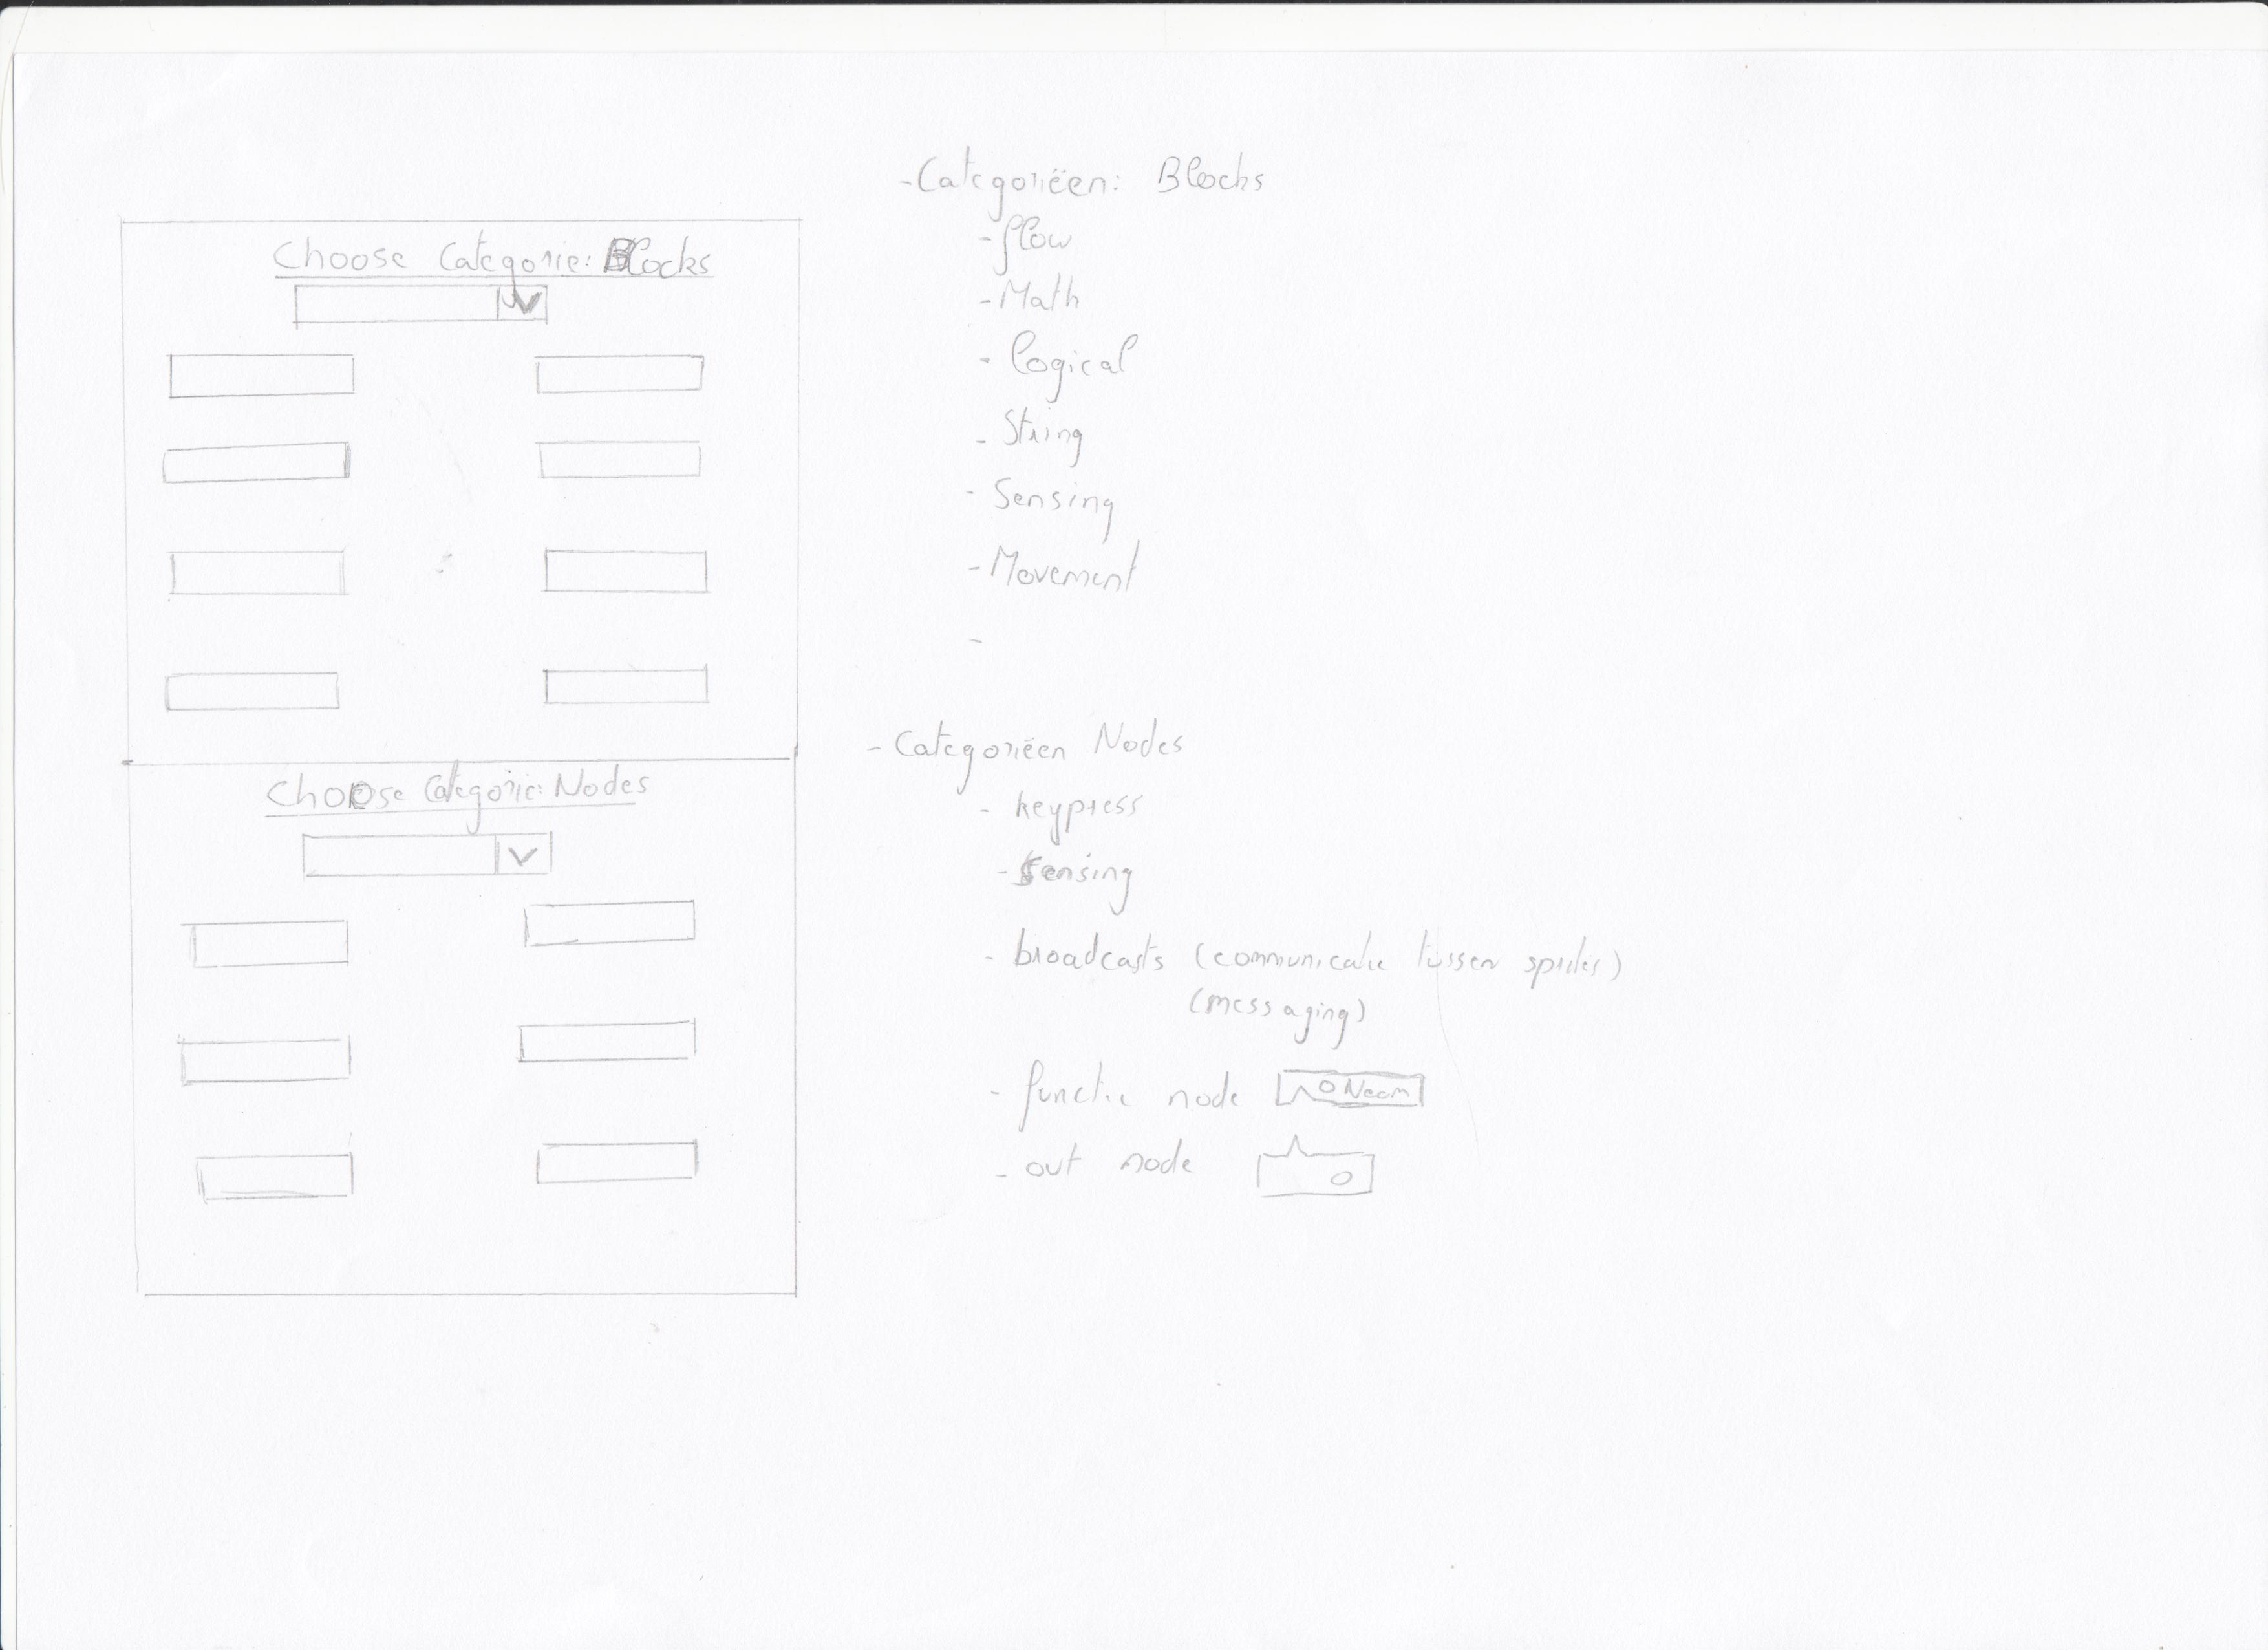
\includegraphics[scale=0.10]{mockup2-4.jpg}
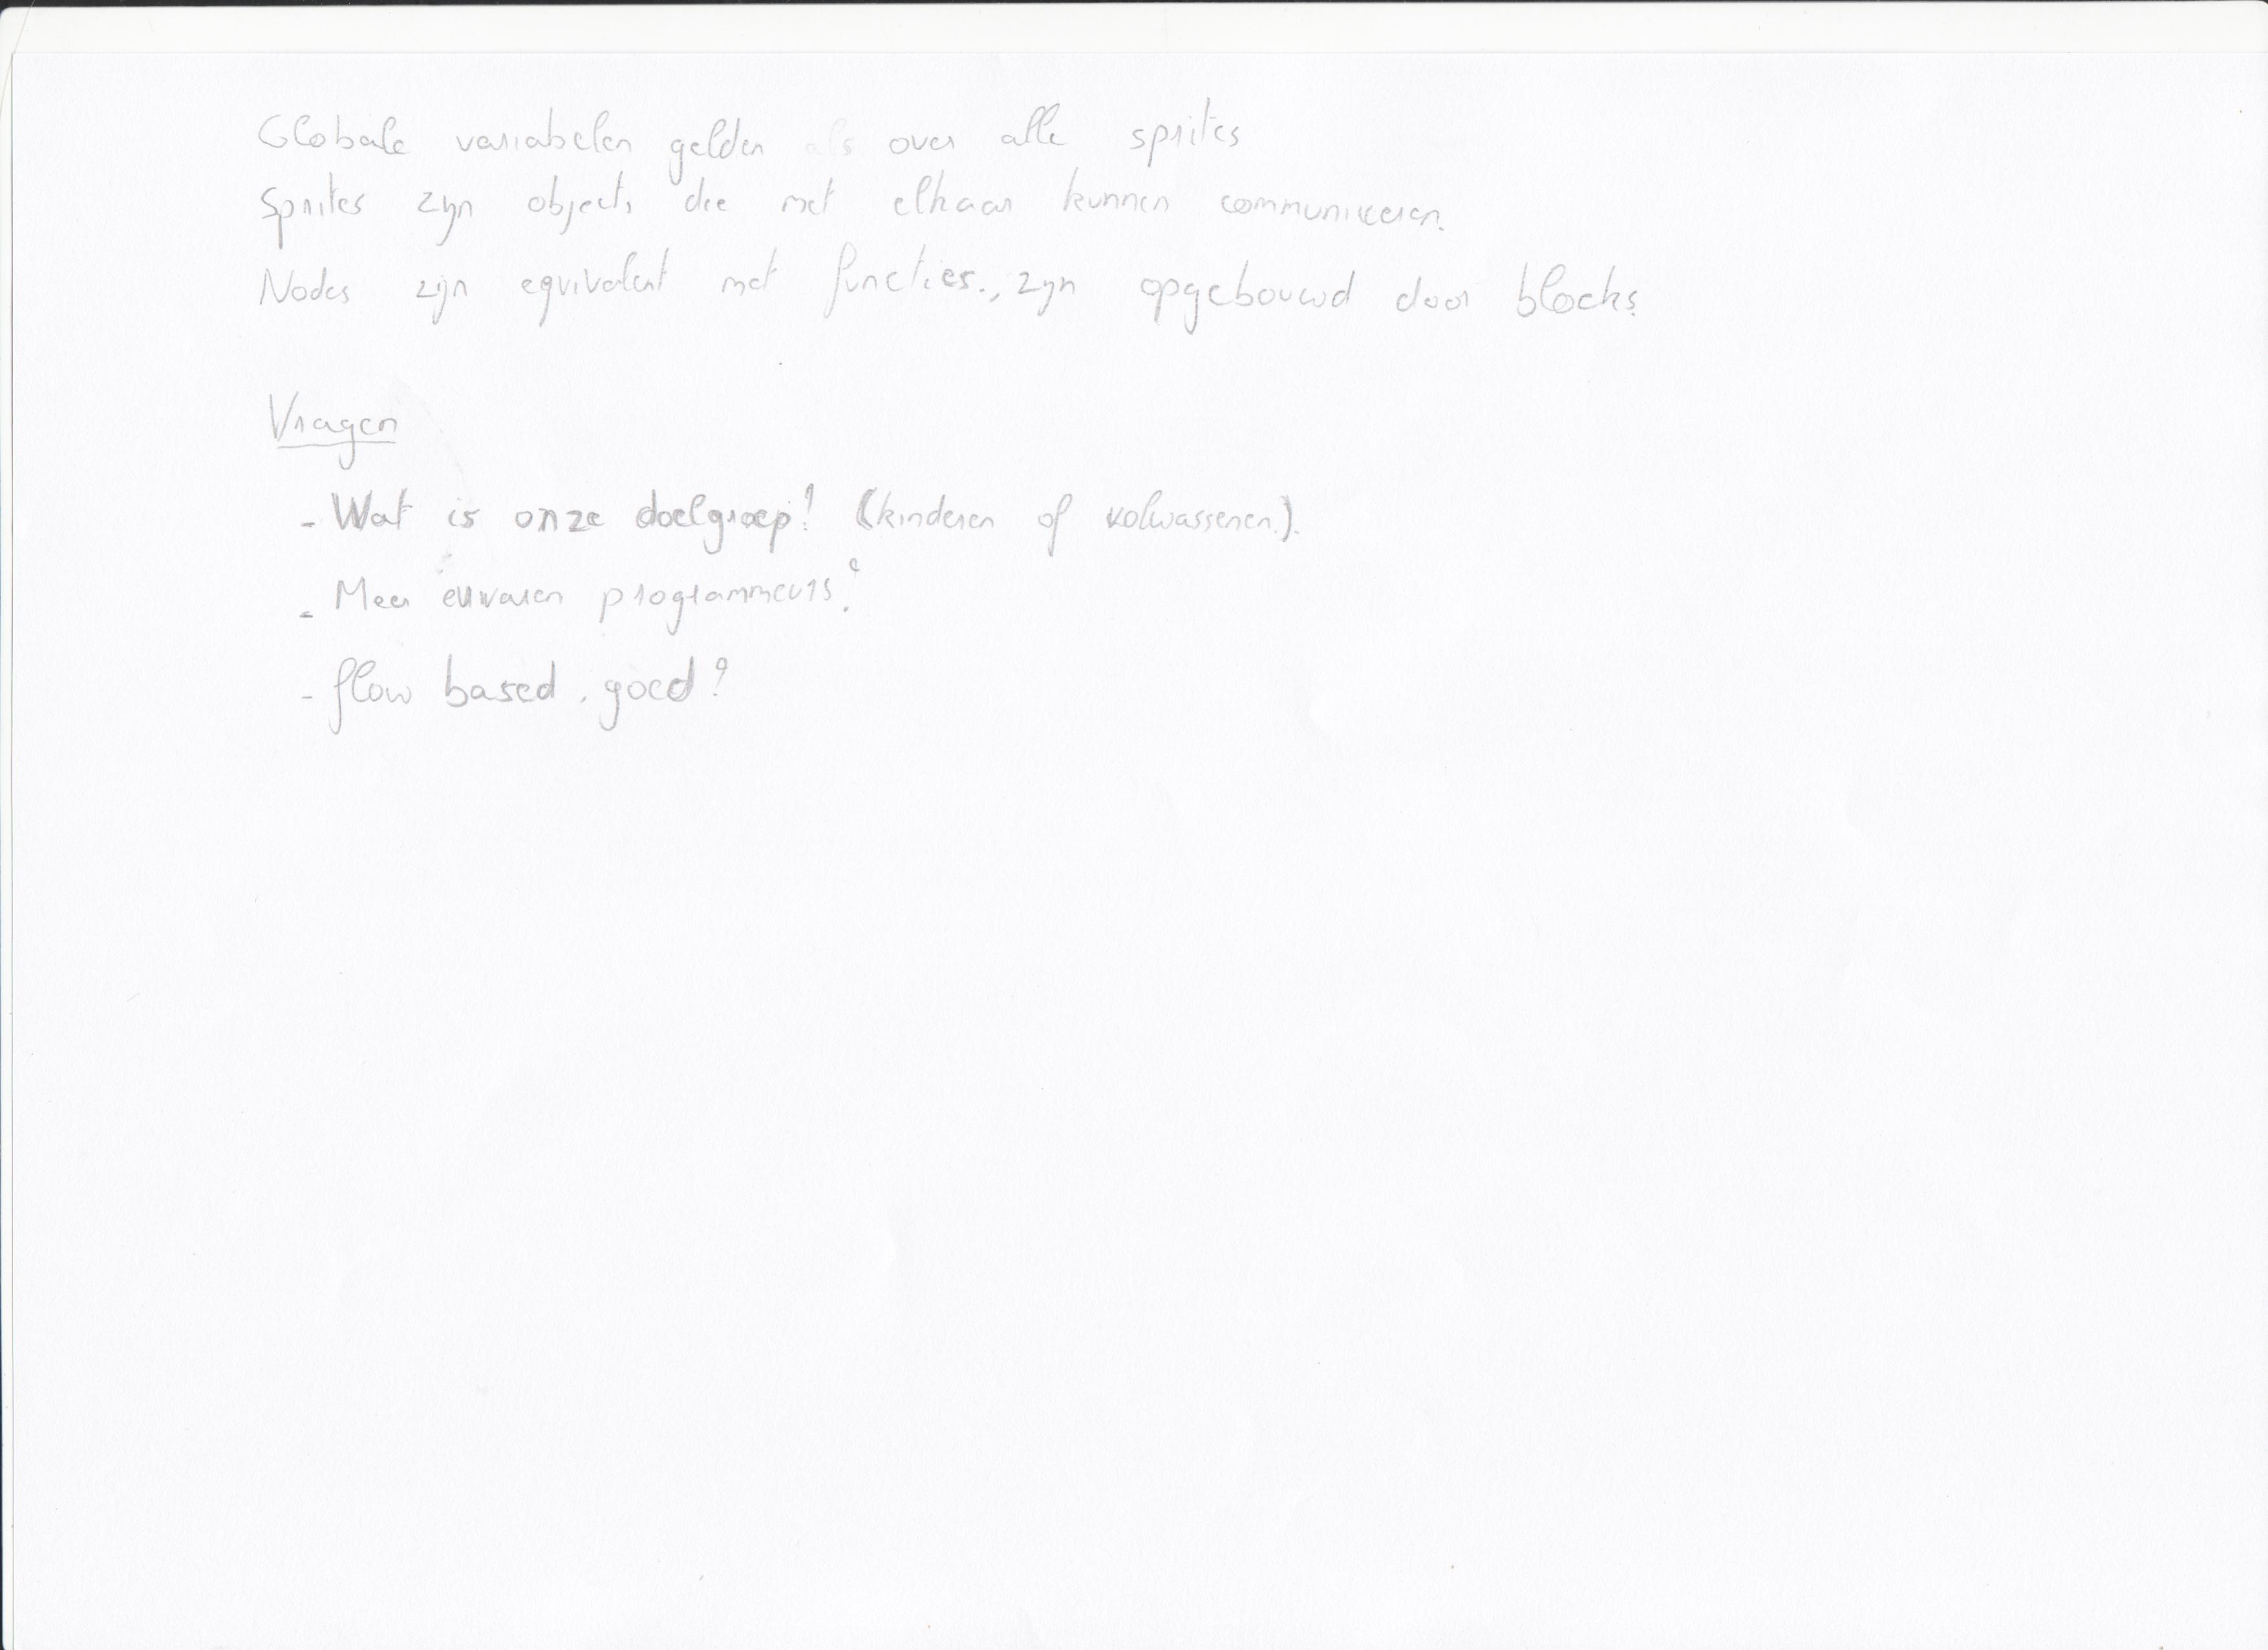
\includegraphics[scale=0.10]{mockup2-3.jpg}

\section{Inhoud van de meeting}
\subsection{Beschrijving van opdrachtgever}
De opdrachtgever Raf Van Ham beschrijft zijn visie over een IDE waarmee een niet technisch persoon gemakkelijk een alarm-systeem mee kan opbouwen. Later werd het duidelijk dat de opdrachtgever een veralgemening in gedachten heeft. Het alarm-systeem is dus echter een voorbeeld van het event-systeem.\\\\
Ons flow-based concept past goed in het idee van de opdrachtgever. Het kan gebruikt worden om componenten (Vb. Drukknop) voor te stellen als nodes. De verbindingen tussen nodes stelt hier het doorgeven van specifieke events voor.\\\\
Events kunnen informatie bevatten zoals een boolean signaal of string (Vb telefoonnummer). Componenten kunnen events triggeren, doorsturen of afhandelen. Events moeten ook terugkoppelbaar zijn om door te geven als ze al dan niet afgehandeld werden. De inhoud van een component moet dus programmeerbaar zijn op een niet technische manier. Er moet de mogelijkheid zijn om nieuwe events en componenten aan te maken.\\\\
Naast de logica tussen componenten moet deze ook fysiek plaatsbaar zijn in een virtuele omgeving. Deze moeten ook getriggerd kunnen worden vanuit de virtuele omgeving.\\\\
Het programma moet een professioneel uitzicht hebben en moet de mogelijkheid bieden om meerder talen te tonen.\\\\
Het gebruikte dataformaat moet leesbaar zijn zodat het handmatig aangepast kan worden. Dit biedt de mogelijkheid om snel scenario's te creeeren. Hiervoor zal waarschijnlijk XML gebuikt worden. Basiscomponenten worden best appart opgeslaan zodat deze herbruikbaar zijn in verschillende projecten.\\\\
Acties van het systeem moeten gelogd worden zodat er een replay modus (Debug modus) mogelijk is. 
 


\end{document}